For each one of the three types of environmental fluctuations and the stable (non-fluctuating) environment (SE) we performed 50 simulations. This produced a total of $4\times50=200$ runs. Each cell of the CA was initialized in a random state, then each cell in one of the 5 living states was initialized with an individual randomly generated genotype. Each run lasted 500,000 iterations under the parameters listed in Table~\ref{settings}.

\begin{table}
\caption{HetCA parameters.}
\footnotesize
\centering
\begin{tabular}{l>{\centering}p{0.2\columnwidth}}\toprule%
Parameter & Value \tabularnewline
\toprule%
Number of living states & 5\tabularnewline
Successive living iterations before decay & 7\tabularnewline
Number of iterations during decay & 375 to 1,875\tabularnewline
Direct transition to decay & enabled\tabularnewline
Size of the grid & 500 $\times$ 500\tabularnewline
Grid boundaries & toroidal grid\tabularnewline
Transition Rule~(TR) & CA-LGP\tabularnewline
Maximum TR size & 50 statmts\tabularnewline
Genotype copy neighborhood  & v.N. (4) \tabularnewline
Transition rule neighborhood & Moore (8)\tabularnewline
\bottomrule%
\end{tabular}
\label{settings}
\end{table}

\subsection{Genotype Size}

We used the number of program statements ($n_\mathrm{prog}$) as a measure of genotype size and computed the average size of all current genotypes of a run every 2,500 iterations. We then reported the average and standard error among all 50 runs sharing the same settings.

\subsection{Phenotype Comparison}

If environmental changes lead to the selection of plasticity or the emergence of phenotypic selections (similar to the EIS) using easily reversible phenotypic mutations \citep{jablonka2014evolution}, then phenotypes from different individuals of the same lineage observed while environmental conditions are similar should be relatively close even though individuals from their lineage evolved in other environmental conditions between these measures. By contrast, if the adaptation to each environmental change is done exclusively through the selection of classical, irreversible genotypic mutations, these phenotypes should be quite different, despite the potential evolutionary convergence. This is why we developed a metric to measure phenotypic proximity between two iterations of the CA. To do this we simply compared the distributions of living cells over the different living states. Thus the phenotypic difference $\sigma(t_1,t_2)$ between two iterations $t_1$ and $t_2$ was calculated as follows:
%
$$\sigma(t_1,t_2) = \sum_{S=1}^5 \abs{ \frac{N(S,t_1)}{N(t_1)}-\frac{N(S,t_2)}{N(t_2)}}$$ 
%
where $N(S,t)$ is the number of cells in living state $S$ at iteration $t$ and $N(t)=\sum_{S=1}^5 N(S,t)$ is the total number of living cells.

Every 5,000 iterations of the CA we performed two phenotypic comparisons between the current iteration $t_1 = t$ and an iteration in the past, $t_2 = t - \Delta t$. In one scenario, the temporal distance $\Delta t$ was a multiple of the periodicity $f$, so that we compared two similar environments: $E(t_1) = E(t_2)$. We chose $\Delta t =$ 60,000 in the SE, ScF and LF cases and 55,000 in the SF case. In another scenario, we introduced an additional single-period shift such that we compared two dissimilar environments: $E(t_1) = E(t_2 + f)$. Here $\Delta t$ was respectively equal to 60,100, 65,000 and 60,000 in the ScF, LF and SF cases.

\subsection{Diversity}

We use the ``true diversity index'' of order two \citep{jost2006entropy} to measure phenotypic and genotypic diversity at every iteration $t$ of the CA. Phenotypic diversity therefore reads:
%
$$^2\!D_p(t)=\left(\sum_{S=1}^5 \left(\frac{N(S,t)}{N(t)}\right)^2\right)^{-1}$$
%
while genotypic diversity is:
%
$$^2\!D_g(t)=\left(\sum_{g=1}^{G(t)} \left(\frac{N(g,t)}{N(t)}\right)^2\right)^{-1}$$
%
where $G(t)$ is the number of distinct genotypes at iteration $t$ and $N(g,t)$ is the number of cells sharing genotype $g$ at iteration $t$. Note that $N(t)=\sum_{S=1}^5 N(S,t)=\sum_{g=1}^{G(t)} N(g,t)$.

\subsection{Homogeneous Test}

We also collected the \emph{most common genotype} (MCG), i.e.~the most frequently occurring one, starting at iteration 2,500, then 102,500 and again every 100,000 steps until iteration 500,000, thus creating 6 sampling points (it was shown by \citet{medernach2015evolutionary} that during the initial iterations of HetCA the MCGs were unlikely to exhibit any viable survival strategy). All MCGs collected in that way were exported and tested alone in homogeneous conditions, i.e. where all cells were initialized with that genotype and no mutations could occur. Since each collected MCG from any one of the four environments (SE, ScF, LF and SF) was tested again in all four environments, we performed a total of $4\times50\times6\times4=4800$ runs. The maximum duration of these runs was set to 60,000 iterations. Sometimes the genotype was not adapted to the environment and all living cells went extinct (i.e. turned to decay or quiescent state) before the end of the simulation. We considered a homogeneity test to be successful if living cells did not go all extinct before 60,000 iterations. In the Results section, we report the success rate of those simulations, along with statistics on the last iterations of the failed runs. 

\subsection{Phenotypic Disturbance in the Homogeneous Test} 

In HetCA, to survive on the long term genotypes must regularly ``release'' cells by transforming them into quiescent cells without genotypes. This generates patterns and cycles easy to observe in homogeneous simulations where a single genotype is tested (Figure~\ref{foursteps}a). It is also observable, although with greater difficulty, in standard heterogeneous HetCA simulations (Figure~\ref{foursteps}b). This is why, to characterize phenotypes we found it useful to measure these cycles as well as their irregularities. At every iteration $t > 8$ of the homogeneous genotype test, we compared the sequence of states $S_t$ and $S_{t-1}$ of each cell to its anterior sequences during the 8 previous iterations of the CA. We assessed whether this sequence of two states was repeated and with what periodicity $p=\min\{p \in [2,7]\}$, i.e.~such that $(S_t,S_{t-1}) = (S_{t-p},S_{t-p-1})$. We used a sequence of two states because, if the genotype of a cell adopts a stable strategy, i.e. repeats a sequence of states, this sequence must contain a minimum of two states in order to ensure the survival of the genotype---the quiescent state and one of the living states. We chose to limit the comparison to the 8 previous iterations in order to reduce the computational cost and because the limit of 7 consecutive live iterations before decay involves, for a successful regular phenotype, a maximum periodicity of 7 iterations for the quiescent state. We performed this measure only if there was at least one living state and no decay among the last two states. We report, for each iteration $t$ of the CA, the phenotypic disturbance
%
$$P(t) = \sum_{p=1}^7 \abs{ \frac{N(p,t)}{N(t)}-\frac{N(p,t-1)}{N(t-1)}}$$
%
where $N(p,t)$ is the total number of cell with periodicity $p$ at iteration $t$. This measure is rough but interesting because, unlike phenotypic differences, it is not directly based on states and therefore is less likely to be correlated to a state’s probability of propagation.
 
\begin{figure}[h]
\centering
\begin{tabular}{cc}
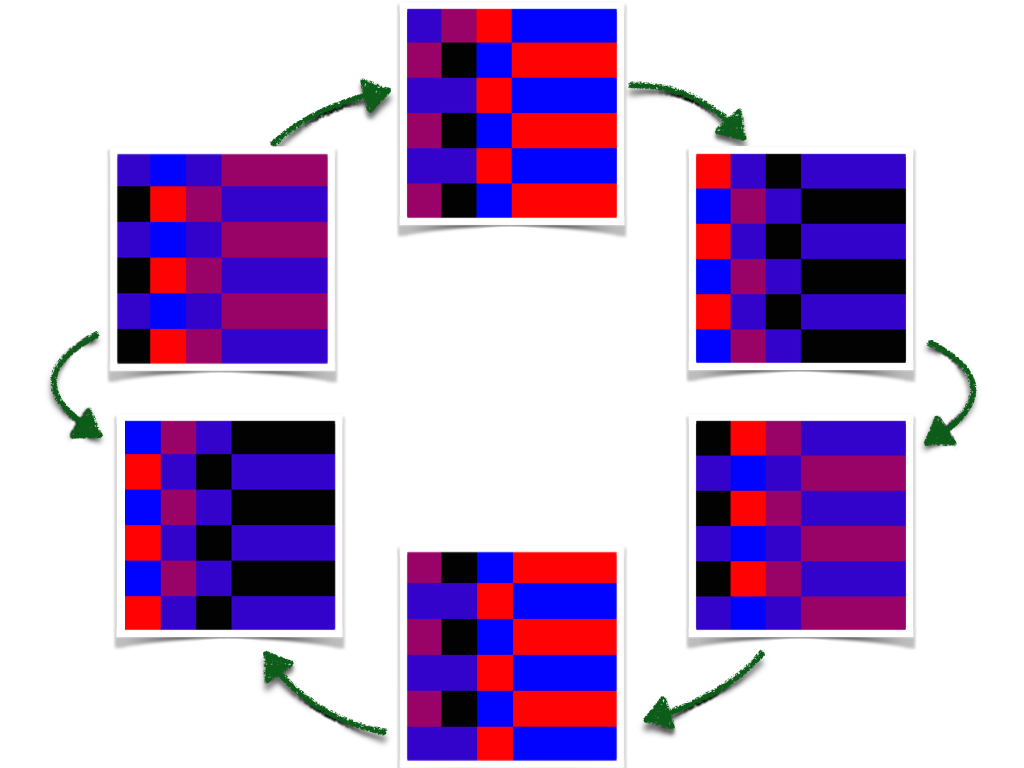
\includegraphics[width=0.45\columnwidth]{img/4steptransition}& 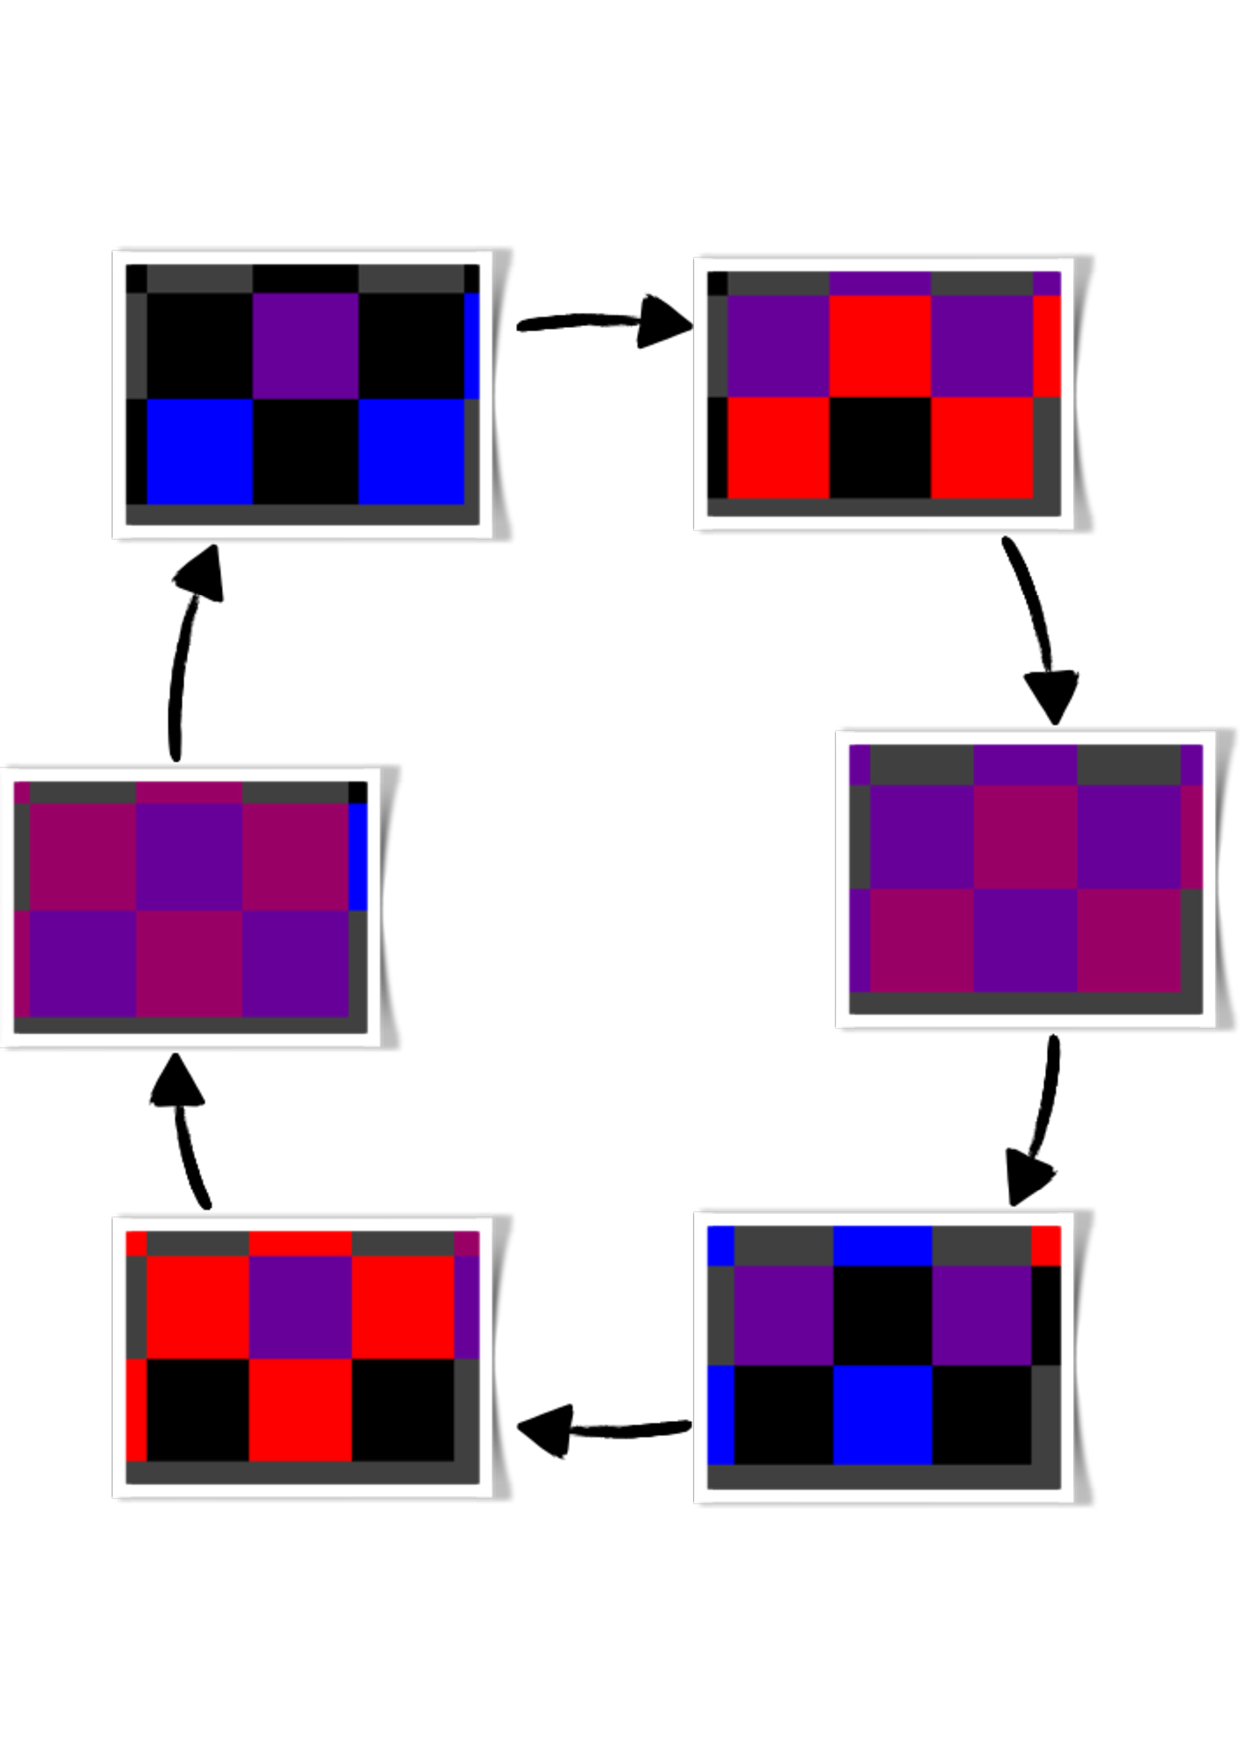
\includegraphics[width=0.45\columnwidth]{img/cyclesReal}\\
(a) & (b)
\end{tabular}
\caption{Examples of 6-step survival strategies: (a) Genotype extracted from a HetCA simulation in a stable environment (SE) with random homogeneous initialization. (b) Genotype produced by short-cycle fluctuations (ScF).}
\label{foursteps}
\end{figure}

%\begin{figure}[h]
%\centering
%\caption{Six steps survival strategy.}
%  \label{fourstepsreal}
%\end{figure}
